\documentclass[10pt,a4paper]{report} 
% Style
\usepackage{amsfonts}
\usepackage{amsmath}
\usepackage{amssymb}
\usepackage[utf8]{inputenc}
\usepackage[T1]{fontenc}
\usepackage[english]{babel}
\usepackage{lmodern} 
\usepackage{graphicx}
\usepackage{color}
\usepackage{float}
\usepackage{url}
\usepackage[numbered]{mcode}

\lstset{extendedchars=\true}
\lstset{inputencoding=ansinew}



% ---Dokumen start---
\begin{document}



% ---Title page ---
\title{Localisation using microphone network\\Sensor fusion -- TSRT14}
\author{Group 12}
\maketitle

\abstract{This is a report for one of the laboration assignments in the course Sensor fusion (TSRT14) at LiTH.
  It consists of estimation, tracking and location for a robot that is moving in a acoustic sensor network.
Several different algorithms are used and compared to each other.}

% ---Innehållsförteckning---
\tableofcontents

\newpage
\chapter{Data gathering}
\label{Data gathering}
The data that is used in this report was gathered during a session at Laboteket.
The setup was a robot that followed a path around a track that was about one meter in diameter.
As the robot went around the track it emitted a pulse two times per second.
The sensors that were used were 7 microphones, that could be placed anywhere around the track.
Three datasets were collected.
First a calibration set. This was collected by placing all the microphones on the same distant from the robot.
This was achived by placing all the microphones on a small segement of a circle with the robot in the center.
The robot was then setup to just emit the pulses and stay still. The setup is displayed in figure \ref{calibtration_setup} below.
\begin{figure}[H]
\begin{center}
  \label{calibtration_setup}
  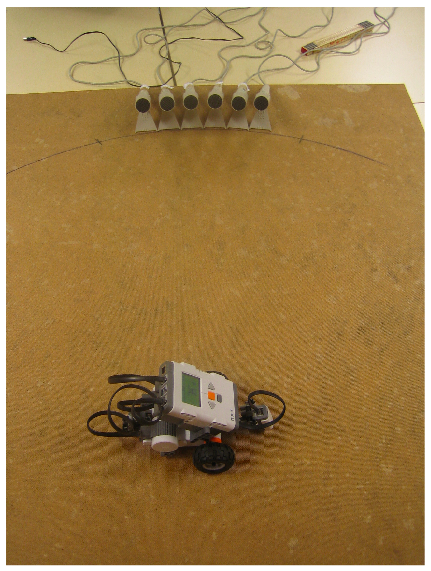
\includegraphics[width = 100pt]{calibration_setup.png}
  \caption{Calibration setup}
  \end{center}
\end{figure}

After this was done the robot was set up to drive around the track while the microphones recorded data.
Two different setup were used. The placement of the microphones can be seen in Figure \ref{good_setup} and \ref{bad_setup}.
The first setup up was chosen to have microphones spread as even as possible around the track.
This will make the arrival times at the microphones as different as possible.
In the second setup the microphones are closer together and there should be less difference between the arrival time of different microphones.

The robot went around the track about two times for each recording session.
The recorded sound was then processed to find the arrival times for each pulse on every microphone.
These arrival times are then used for tracking and localisation.

The processing of the recordings are done by correlating the recorded signal with the pulse that was transmitted from the robot.
This will give large peaks where the pulses were recorded.
There is still a problem with this approach, the pu

\begin{figure}[!h]

  \label{good_setup}
  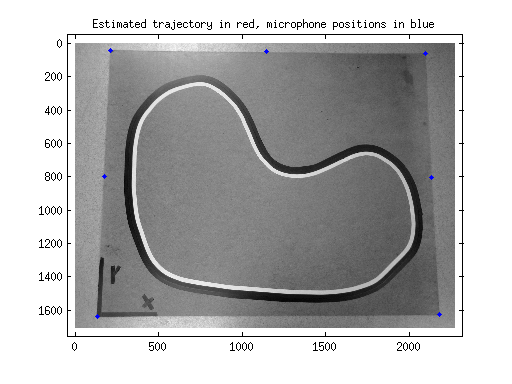
\includegraphics[scale=0.9]{microphone_pos_good.png}
  \caption{Microphone setup one.}
\end{figure}

\begin{figure}[!h]
  \label{bad_setup}
  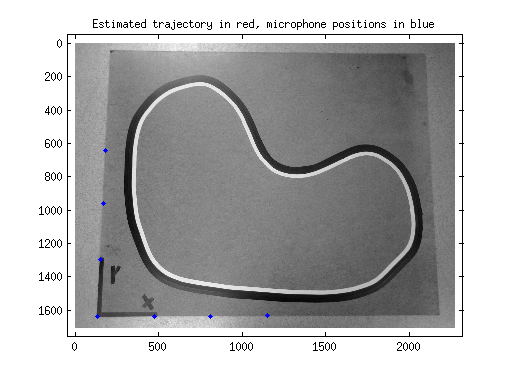
\includegraphics[scale=0.9]{microphone_pos_bad.png}
  \caption{Microphone setup two.}
\end{figure}

\newpage
\chapter{Tasks}
\label{Tasks}

\newpage
\section{Calibration}
\label{Calibration}
The calibration setup described in chapter \ref{Data gathering} in figure \ref{calibtration_setup} produced data which contained the arrival time at each time instant for each sensor. To determine the accuracy of the measurement, the bias and standard deviation is needed. First the error is calculated. Example code for one sensor is shown in the following matlab code. 
\begin{verbatim}
e = tphat(:,1) - mean(tphat, 2);
\end{verbatim}
The same has to be done for the other 6 sensors. The meaning of this is that the mean of the seven sensors at one time instant should be close to the actual value of the arrival time. Since they are placed at en equal distance the arrival time should be the same, but since they are not, we need to compare the measurements to the mean of the sensors, which produces the error.

To compare the empirical probability density function of the measurement noise with a pdfclass distribution, we need to compute a normalized histogram first. This can be achieved using the following code.
\begin{verbatim}
bias = [];
std_deviation = [];
P = [];
mu = [];

figure()
for i = 1:nr_of_sensors
    [N,l] = hist(e(:,i),20);
    Wb = l(2)-l(1); %bin width
    Ny = length(e(:,i)); %nr of samples
    subplot(2,4,i)
    bar(l,N/(Ny*Wb));
    d = i+1;
    title(sprintf( 'Sensor %d', d));
    hold on
    pe_i = ndist(mean(e(:,i)), var(e(:,i)));
    mu = [mu; pe_i.mu];
    P = [P pe_i.P];
    plot(pe_i);
    hold off
    bias = [bias mean(e(:,i))]; % [m] Bias för alla sensorer
    std_deviation = [std_deviation sqrt(var(e(:,i)))];
end
\end{verbatim}
This code also plotts a pdfclass distribution into the same graph for comparison. It also determines the bias and standard deviation for each sensor. 
\begin{figure}[H]
  \label{histogram}
  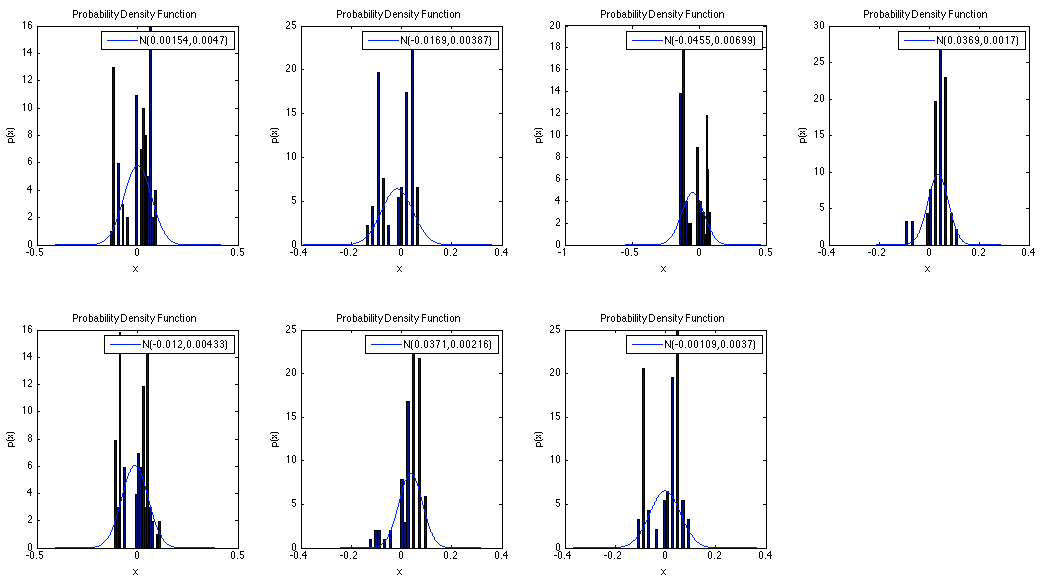
\includegraphics[width = 400pt]{histogram.png}
  \caption{Histogram and pdfclass distribution for each sensor}
\end{figure}
The mean of the standard deviatione is $0.0613$ meters, which can be regarded as the accuracy of the estimation.



\newpage
\section{Sensor modelling}
\label{Sensor modeling}

\newpage
\section{Experiments}
\label{Experiments}

\newpage
\section{Configuration analysis}
\label{Configuration analysis}

\newpage
\section{Localisation}
\label{Localisationg}

\newpage
\section{Tracking}
\label{Tracking}

\newpage
\section{Sensitivity analysis}
\label{Sensitivity analysis}

\chapter{Appendix}
% .m code

\end{document}



%%% Local Variables: 
%%% TeX-PDF-mode: t 
%%% TeX-master: "rapport"
%%% End: 

